\documentclass{ieeeaccess}
\usepackage{cite}
\usepackage{amsmath,amssymb,amsfonts}
\usepackage{algorithm,algorithmic}
\usepackage{cases}
\usepackage{empheq}
\usepackage{graphicx}
\usepackage{textcomp}
%\usepackage{natbib}

\def\BibTeX{{\rm B\kern-.05em{\sc i\kern-.025em b}\kern-.08em
    T\kern-.1667em\lower.7ex\hbox{E}\kern-.125emX}}
\begin{document}
\history{Date of publication xxxx 00, 0000, date of current version xxxx 00, 0000.}
\doi{10.1109/ACCESS.2017.DOI}

\title{An Energy Efficient D2D-Aided User Scheduling Scheme for Maritime Communications}
\author{\uppercase{Yunzhong Hou}\authorrefmark{1}, 
\uppercase{Te Wei}\authorrefmark{1}, \IEEEmembership{Student Member, IEEE},\\
\uppercase{Wei Feng}\authorrefmark{1}, \IEEEmembership{Member, IEEE}, 
\uppercase{Ning Ge}\authorrefmark{1}, \IEEEmembership{Member, IEEE},
\\ \uppercase{and Jianhua Lu}\authorrefmark{1}, \IEEEmembership{Fellow, IEEE}}

\address[1]{Tsinghua National Laboratory for Information Science and Technology, Tsinghua University, Beijing 100084, P. R. China}

\tfootnote{This work was partially supported by the National Basic Research Program of China under grant No. 2013CB329001, and
the National Science Foundation of China under grant No. 91638205 and grant No. 61621091. The authors Yunzhong Hou and Te Wei contributed equally to this work.}

\markboth
{Hou \headeretal: An Energy Efficient D2D-Aided User Scheduling Scheme for Maritime Communications}
{Hou \headeretal: An Energy Efficient D2D-Aided User Scheduling Scheme for Maritime Communications}

\corresp{Corresponding author: Yunzhong Hou (e-mail: houyz14@mails.tsinghua.edu.cn).}

\begin{abstract}

Energy consumption reduction is a critical issue for maritime communication systems. 
In this paper, we reduce the energy consumption by making channel estimation and implementing D2D transmission, which introduce the time dimension and transmitter (BS/relay) dimension in our optimization subspace respectively. Together with the receiver (user) dimension which has been studied previously, our optimization subspace becomes 3-dimensional and therefore provides great potential. 
Since the wireless channels are time-varying, it is impossible to accurately predict the complete channel state information (CSI). We exploit the positional information of each vessel based on its specific shipping lane and timetable. Utilizing the positional information, we replace the complete CSI with the slowly-varying large-scale channel fading estimation. Besides, we particularly focus on the delay-tolerant information distribution service, and implement D2D transmission for further improvement energy-wise. 
On that basis, we decompose the NP-hard energy consumption optimization problem into 3 subproblems. We propose an efficient algorithm for each subproblem in an iterative way with a polynomial time complexity. 
Simulation results justify our large-scale CSI estimation and reveal that the proposed D2D-aided process-oriented scheme significantly reduces the energy consumption by up to 50\% over the cellular-only ones, benefiting from higher dimensional optimization subspace.

\end{abstract}

\begin{keywords}
Process-oriented, maritime communications, user scheduling, large-scale channel fading estimation, D2D
\end{keywords}

\titlepgskip=-15pt

\maketitle

\section{Introduction}
\IEEEPARstart{W}{ith} the rapid development of marine activities such as marine tourism, offshore aquaculture and oceanic mineral exploration, the demand for reliable and high-speed maritime communication services increases sharply. Oceanic economic and cultural exchanges between countries, such as the Maritime Silk Road project in China, have further promoted this demand \cite{p322}\cite{p101}. In order to meet the increasing demand, several maritime communication network (MCN) projects have been developed in recent years, e.g., the BLUECOM+ project, the MarCom project, and the TRITON project \cite{p321}--\cite{p32}.
Unlike terrestrial cellular networks, a maritime communication system has quite limited geographically available base station (BS) sites. In order to cover a vast area with limited BSs, the system usually adopts high-powered BSs, which increases the operational costs of mobile network operators and poses a global threat to the environment \cite{p33}.
Accordingly, reducing energy consumption becomes a critical issue for maritime communications.
Device-to-device (D2D) communication underlaid with cellular networks allows direct communication between mobile users \cite{p3331}-\cite{p3333}. With proximate communication opportunities, D2D communication may increase spectral efficiency, improve cellular coverage, as well as reduce energy consumption.
Therefore, advanced wireless transmission and radio resource management techniques for D2D underlaid cellular communication system are in urgent need to solve the maritime power reduction problem.


\subsection{Related work}
%cellular
So far, energy-efficient user scheduling techniques have been extensively studied for terrestrial cellular networks, such as the proportional fairness based schemes in \cite{p61}--\cite{p63}, the signal-to-leakage-interference-plus-noise ratio based methods in \cite{p64}--\cite{p66}, the coordinated scheduling with cyclic beamforming in \cite{p67}\cite{p68}, and the iterative algorithms in \cite{p69}\cite{p70}. Based on the utilization degree of CSI, user scheduling schemes can be classified into three categories. The first one required no CSI, such as the simple but efficient round-robin scheme for fair queuing \cite{p51}. The second one exploited statistical and outdated CSI, as studied in \cite{p52} and \cite{p53}. The third one assumed full CSI, and utilized the instantaneous CSI for user scheduling in a minuscule time scale, i.e., in each coherence time \cite{p3}--\cite{p7}. In \cite{p3}, a joint antenna-subcarrier-power allocation scheme was proposed for distributed antenna systems with limited backhaul capacity to maximize the energy efficiency while providing min-rate guaranteed services. In \cite{p6}, a matching algorithm of joint sub-channel assignment and power allocation was developed for non-orthogonal multiple access networks to maximize the total sum-rate with user fairness taken into consideration. In \cite{p4}, a joint power allocation and user scheduling algorithm based on dynamic programming (DP) was proposed for multi-user MIMO systems to minimize the total energy consumption under hard delay constraints. In \cite{p5}, a cross-layer cooperative user scheduling and power allocation scheme was developed for hybrid-delay services, and the fundamental tradeoff between delay and energy consumption was illustrated. More recently in \cite{p7}, a user scheduling and pilot assignment scheme was proposed for massive MIMO systems to serve the maximum number of users with guaranteed QoS.

%D2D
There are also several power control scheme developed for terrestrial D2D underlaid cellular systems so far. Xiao et al. proposed a power optimization scheme with joint resource (i.e. subcarrier and bit allocation) allocation and mode selection in an OFDMA system with integrated D2D communications in \cite{p801}. In \cite{p802}, Lee et al. proposed a random network model for a D2D underlaid cellular system using stochastic geometry and developed centralized and distributed power control algorithms. \cite{p801} and \cite{p802} assumed full CSI, which is used for user scheduling in coherence time. In \cite{p803}, a distributed power control algorithm was developed which iteratively determines the SINR receivers in a mixed cellular and D2D environment and allocates transmit powers such that the overall power consumption is minimized subject to a sum-rate constraint. In \cite{p804}, a power-efficient mode selection and power allocation scheme in D2D underlaid cellular system was developed which based on exhaustive search of all possible mode combinations of the devices.  

%问题

%信道
However, in maritime scenarios, the wireless channel model becomes totally different. Unlike terrestrial scenarios, obtaining accurate instantaneous CSI in maritime communications becomes problematic due to the large propagation delay, whereas using large-scale CSI such as the location information will be more feasible. As a result, a new user scheduling scheme based on large-scale CSI, which is able to exploit specific properties of maritime wireless channels, should be designed. To the best of the authors' knowledge, few user scheduling schemes specific to maritime channels have been reported in the literature, and the system performance with only the large-scale CSI has not been sufficiently studied either. 

As both the wireless channels and the users' demands are time-varying, long-term predictions are in general very challenging. Therefore, all the above user scheduling schemes are based on the CSI and service requirements in a short time scale, e.g., in the scale of the coherence time ($\mu$s) or several time slots (ms). The duration of the service, however, can last for several seconds, minutes or more. That is to say, these schemes, without considering the long-term CSI during the service process, lose the potential gain that could be achieved by enlarging optimization space in the time dimension. These optimizations in the above cellular-only studies are in 1-dimensional subspaces, i.e. receiver (user) dimension, as they are based on CSI of a short time period and have only one transmitter, the BS. 

%D2D-海域需求不同
Current energy-efficient D2D user scheduling study mainly focused on terrestrial scenarios. Given the uncertainty and volatility in terrestrial users' service requirements, the D2D user scheduling in current studies has to be finished within a short period of time in order to keep update with the QoS need changes. Besides, in terrestrial scenarios, the CSI can be easily acquired instantaneously, which makes it easy to complete the user scheduling process within that short period of time. 
Whereas in maritime scenarios, service requirements differ greatly. Users or ships pay more attention to reliability and data amount rather than service delay. Moreover, instantaneous CSI is difficult to acquire under high propagation delay in maritime scenarios. As a result, current terrestrial D2D user scheduling schemes are unfit for maritime scenarios. 

Nevertheless, implementing D2D transmission in maritime cellular data-distribution system can bring forward great improvements energy-wise, as the introduction of D2D came along with a new dimension in optimization subspace. Since users can  act like relays in D2D scenarios, and can be further regarded as transmitter in data transmission, introducing D2D transmission to cellular-only systems can bring forward a new dimension: the transmitter (BS/relay) dimension. Current D2D user scheduling optimize in a 2-dimensional subspace, one transmitter (BS/relay) dimension and one receiver (user) dimension, but unable to dig into the time dimension. Hence, a D2D user scheduling scheme focused on maritime specified service requirements and channel characteristics is needed. This time, considering the long-time CSI and delay-tolerant service requirements, the D2D user scheduling can benefit more from the yet-to-explore time dimension. 


%All of the above user scheduling schemes, cellular, and the optimization is in a ${\left( {J + 1} \right) \times J}$ 2-dimensional subspace (user count $J$). As the service process information is ignored, the state-oriented schemes lose the potential gain in energy efficiency to a great extent, especially for maritime vessels with dynamic locations and service requirements.
%In our previous study \cite{p108}, a process-oriented user scheduling scheme for maritime cellular-only communication system was developed. The optimization in \cite{p108} was in a  ${J \times T}$ 2-dimensional subspace (time slot count $T$).

\subsection{Contributions}


In this paper, we further explore a 3-dimensional optimization subspace, including one transmitter (BS/relay) dimension, inspired by terrestrial D2D communications; one receiver dimension; and one time dimension, as we make channel estimation by utilizing the service process information, which has not been considered in the previous studies. Through enlarging the optimization subspace, we reduce the energy consumption for maritime D2D underlaid cellular communications. 

Apart from D2D user scheduling, the major challenge for our proposed scheme lies in the long-term prediction of the CSI, as well as the prediction of the users' requirements. We overcome these difficulties by fully utilizing the following unique features of maritime communications:

\textbf{(1)} As there are fewer scatterers on the sea than that in the terrestrial scenario, we exploit the position information of marine users to estimate and predict the slowly-varying large-scale CSI instead of the complete instantaneous CSI;

\textbf{(2)} The users' positions can be predicted based on their specific shipping lanes and timetables;

\textbf{(3)} Besides, we particularly focus on the delay-tolerant information distribution service, which is initiated and terminated when a marine user sails into and out of the BS's coverage, respectively, so that we can make long-term prediction of the users' requirements.

% maritime

Given the delay tolerant characteristic of maritime communication: mobile users focus more on reliability and data volume of cellular download rather than transmission delay, we can sacrifice delay for larger system capacity and less energy consumption. 
%Hence we focus on the delay-tolerant information distribution service in this study.
Since the shipping lanes of maritime mobile users are acquired beforehand, we can use the shipping lanes to predict long-time user locations. And the user locations are of great use in determining the long-time large-scale channel fading, according to the scarcity of scatterers on the sea, which makes it easier to estimate and predict the slowly-varying large-scale channel fading. Therefore, we exploit the positional information of each vessel based on its specific shipping lane and timetable to estimate the large-scale channel fading instead of the complete CSI, as the research in \cite{p120} suggests that large-scale channel fading is a good estimate for the complete CSI. %冯伟老师文章
With delay-tolerant service assumption and large-scale channel fading estimation, we address the user requirement problem and the CSI prediction problem based on the characteristic of maritime communication system. On that basis, we enlarge the optimization subspace by introducing the time dimension. 

% d2d
Since we focus on energy consumption of a maritime data-distribution system, the implementation of D2D communication can be of great help since its superiority in energy consumption, spectral efficiency and cellular coverage. Inspired by terrestrial D2D communication, we introduce the transmitter dimension (BS/relay) in our maritime user scheduling optimization subspace. With the increment of time dimension and transmitter dimension, our D2D-aided user scheduling scheme and explore the 3-dimensional optimization subspace for energy consumption improvement rather than the 1-dimensional (receiver dimension only) optimization subspace in traditional cellular-only method. 


% proposed method

In this paper, we formulate a energy consumption optimization problem for D2D-aided user scheduling, aiming to minimize the energy consumption while providing users with delay tolerant data distribution services. The problem is proved to be NP-hard. To overcome the difficulties of solving the NP-hard problem, we enlarge the optimization subspace into 3-dimensional and decompose the problem into three simpler subproblems. We further propose efficient algorithms to solve the subproblems in an iterative way with a polynomial time complexity.
Simulation results reveal that the proposed process-oriented D2D-aided scheme in a 3-dimensional optimization subspace significantly outperforms the state-oriented ones in terms of energy consumption by taking advantage of the service process information and cellular-\&-D2D routes, and the impact of the small-scale channel fading is neglectable. 


\subsection{Organization and Notation}
%文章组织
The rest of the paper is organized as follows.

Section II introduces the system model, where a multi-user maritime communication system is considered in the presence of D2D transmissions, and the formulation of the optimization problem for user scheduling is presented.
In Section III,  the problem is decomposed into three subproblems and solved in an iterative way.
Section IV presents simulation results along with further discussions.
Finally, Section V gives the concluding remarks.

Throughout this paper, lightface symbols represent scalars, while boldface symbols denote vectors and matrices. ${\mathbf{I}}_{M \times N}$ represents an ${M \times N}$ identity matrix, $\mathbb{E}[x]$ denote the expectation of $x$, and $\mathcal{CN}(0, {\sigma}^2)$ denotes the complex Gaussian distribution with zero mean and ${\sigma}^2$ variance. 
%$[x]^{+}\triangleq{\mathop {\max }(x,0)}$. $\lfloor x \rfloor$ and $\lceil x \rceil$ denote the largest integer not greater than $x$ and the smallest integer not less than $x$, respectively. ${\mathbf{A}}^T$ and ${\mathbf{A}}^H$ represent the transpose and the transpose conjugate of ${\mathbf{A}}$, respectively. 



\section{System Model}



\begin{figure} [htb]
\includegraphics*[width=8.8cm]{SysModel.png}
\caption{Maritime communication system for information distribution service.}\label{fig:1}
\end{figure}


%\Figure[t!](topskip=0pt, botskip=0pt, midskip=0pt){SysModel.eps}
%{Maritime communication system for information distribution service.\label{fig1}}

As shown in Figure 1, the following sections focus on the D2D underlaid cellular downlink transmission of a single-cell maritime communication system. In the system there are one onshore BS
% equipped with $L$ antennas 
and  $J$ single-antenna users (ships) in the sea. We assume that there are $N$ subcarriers, and the subcarrier bandwidth is ${B_s}$. 

In the studied system, D2D communications between ships use the same licensed band of cellular network (i.e. one of the $N$ subcarriers), and the same air interface of the underlying cellular communication. As a result, D2D communications consumes part of the resources allocated to the cellular network.
%, i.e., D2D communications also use the $N$ subcarriers whose bandwidths are ${B_s}$. 
At any given time, each D2D or cellular transmission route will use distinct subcarrier. Here in this paper by `route' we mean the transmission from BS/relay to user during a certain time period. We further assume that the $J$ single-antenna users can either receive data from one transmitter (BS/relay) or send data to another user (act as a relay) at any given time.

Without loss of generality, we assume the cell shape to be a semicircle. 
% with radius $R$. 
Each user sails into and out of the cell according to its shipping lane and timetable. For each user, delay-torrent service is assumed, and the total amount of the data required by the ${j^{th}}$ user is denoted by $C_j^{QoS}$. In order to simplify the problem, we only consider D2D and cellular communications of the ships in the semicircle. We also assume all the users request different data and the system has no D2D data reuse.

We further assume a modified 2-ray propagation model, since the sea surface is relatively flat. For a given subcarrier, we denote the composite channel gain from the BS/relay $i$ to the user $j$ at time slot $t$ by $\sqrt {{\beta _{i,j,t}}} {h_{i,j,t}}$. The small-scale fading vectors ${h_{i,j,t}}$ follows a complex Gaussian distribution with standard deviation ${\sigma _s} = 1$, i.e., ${h_{i,j,t}} \sim \mathcal{CN}(0, \mathbf{I})$. The large-scale fading coefficient ${\beta _{i,j,t}}$ is expressed as \cite{p0}--\cite{p2}
\begin{align}
{\beta _{i,j,t}} = {\left( {\frac{\lambda }{{4\pi {d_{i,j,t}}}}} \right)^2}{\left[ {2\sin \left( {\frac{{2\pi {h_t}{h_r}}}{{\lambda {d_{i,j,t}}}}} \right)} \right]^2}
\end{align}
where $\lambda $ is the carrier wavelength, ${d_{i,j,t}}$ is the distance between the BS/relay $i$ and the user $j$ at time slot $t$. The antenna height of the transmitter and the receiver are represented by $h_t$ and $h_r$ respectively.

In this paper we proposed a slowly-varying large-scale CSI estimation for the channel under low SNR as shown below in (2a)-(2c). We justify our approximation by simulations in Section IV. SIMULATION RESULTS. Denote ${\gamma _{i,j,t}} = {\raise0.7ex\hbox{${{P_{i,j,t}}{\beta _{i,j,t}}}$} \!\mathord{\left/
 {\vphantom {{{P_{i,j,t}}{\beta _{i,j,t}}} {{\sigma ^2}}}}\right.\kern-\nulldelimiterspace}
\!\lower0.7ex\hbox{${{\sigma ^2}}$}}$ for simplicity, the channel capacity or transmission speed in this paper can therefore be simplified

\begin{subequations}
\begin{align}
{r_{i,j,t}} & = {\mathbb{E}}\left [ {{B_s}{{\log }_2}\left( {1 + \frac{{{P_{i,j,t}}{\beta _{i,j,t}}{{\left| {{h_{i,j,t}}} \right|}^2}}}{{{\sigma ^2}}}} \right)} \right ] \\
& = {\mathbb{E}}\left [  {B_s}{\log }_2 \left( {1 + {\gamma _{i,j,t}}{{\left| {{h_{i,j,t}}} \right|}^2}} \right)  \right ] \\
& \approx \left( {{{\log }_2}e} \right){e^{\frac{1}{{{\gamma _{i,j,t}}}}}}\int_1^\infty  {\frac{1}{u}{e^{ - \frac{u}{{{\gamma _{i,j,t}}}}}}du} 
\end{align}
\end{subequations}

%here in (4) ${{\mathbb{E}}\left [ {{{\left| {{h_{i,j,t}}} \right|}^2}} \right ] = \left| {{h_0}} \right|^2} = 1$ represents the variance of the zero-mean small-scale fading vector ${h_{i,j,t}}$. 
By taking out the expectation operator, we complete our slowly-varying large-scale CSI estimation of complete channel in (2c). Any further denotation of CSI in this paper refer to the `slowly-varying large-scale CSI estimation' unless specified. The impact of this estimation is further discussed in Section IV. SIMULATION RESULTS.

To fully utilize the slowly-varying characteristic of the large-scale channel fading, we divide the total service time into $T$ time slots, each lasts $\Delta t$. The value $\Delta t$ is carefully chosen so that $\beta _{i,j,t}$ remains constant in each time slot $t$. Thus, we make it possible to estimate $\beta _{i,j,t}$ for $\forall t \in \left\{ {1,...,T} \right\}$ based on shipping lanes and timetable. With the large-scale channel fading (CSI) known beforehand, we can further design and implement a process-oriented scheme foe user scheduling.

The total energy consumption of the system consists of cellular transmission part and D2D transmission part. The energy consumption in this system is

\begin{align}
{{E_{total}} = \sum\limits_{j = 1}^J {{E_j}}  = \sum\limits_{j = 1}^J {\left( {\sum\limits_{t = 1}^T {\sum\limits_{i = 0}^J {{P_{i,j,t}}\Delta t} } } \right)} }
\end{align}
here ${P_{i,j,t}}$ represents the average power consumed by the transmission from BS/relay $i$ to user $j$ during time slot $t$.

Our objective is to minimize the system energy consumption by means of user scheduling in cellular transmission and D2D transmission. We further denote the transmission route from BS/relay $i \in \left\{ {0,1,...,J} \right\}$($i = 0$ means BS, $i > 0$ means user relay) to user $j$ at time slot $t$ by $i \to j@t$. For the transmission route $i \to j@t$, we denote the ratio of used transmission power to max transmission power by 

\begin{align}
{{\eta _{i,j,t}} = \frac{{{P_{i,j,t}}}}{{P_i^{\max }}},{\eta _{i,j,t}} \in \left[ {0,1} \right]}
\end{align}
${\eta _{i,j,t}} = 0$ means there is no transmission from BS/relay $i$ to user $j$ at time slot $t$, while ${\eta _{i,j,t}} \in \left( {0,1} \right]$ means a subcarrier is scheduled at time slot $t$ for the transmission and the transmission uses ${\eta _{i,j,t}}$ of the transmitter's max transmission power. $P_i^{\max } = \left\{ {P_0^{\max },\left\{ {P_j^{\max }} \right\}} \right\}$ represents the maximum transmission power of BS or relays. 

By ${C_{j,t}}$ we denote the total data volume user $j$ currently has at time slot $t$. Since the system has no D2D data reuse, user $j$ must have enough data ${C_{j,t}}$ in order to act as relay and transmit to another user $j'$ at $t$

Thus, we formulate the \textbf{energy consumption optimization problem} as

\begin{subequations}
\begin{align}
& \mathop {\min }\limits_{{\mathbf{{\rm H}}} \in {{\left[ {0,1} \right]}^{\left( {J + 1} \right) \times J \times T}}} \left\{ {\sum\limits_{t = 1}^T {\sum\limits_{j = 1}^J {\sum\limits_{i = 0}^J {{P_{i,j,t}}\Delta t} \,} } } \right\} \\
& {s.t.} \;\; \sum\limits_{i \ne j} {\left( {{\eta _{i,j,t}} > 0} \right)}  + \sum\limits_{j' \ne j} {\left( {{\eta _{j,j',t}} > 0} \right) \le {\text{1}}} \\
& \;\;\;\;\;\; \sum\limits_j {\sum\limits_i {\left( {{\eta _{i,j,t}} > 0} \right)} }  \le N \\
& \;\;\;\;\;\; {\left. {{{\left. {{C_{j,t}}} \right|}_{t = 0}} = 0, {C_{j,t}}} \right|_{t = T}} \ge C_j^{QoS} \\
& \;\;\;\;\;\; {C_{j,t}} = \sum\limits_{\tau  = 1}^t {\left( {\sum\limits_i {{r_{i,j,\tau }}}  - \sum\limits_{j'} {{r_{j,j',\tau }}} } \right)\Delta t} ,\; {C_{j,t}} \ge 0
\end{align}
\end{subequations}
${\mathbf{{\rm H}}}{\text{ = }}{\left\{ {{\eta _{i,j,t}}} \right\}^{\left( {J + 1} \right) \times J \times T}}$ since we have to consider transmissions from ${J + 1}$ transmitters (BS/relays) to $J$ receivers (users) at $T$ time slots, and our optimization is in a $\left( {J + 1} \right) \times J \times T$ 3-dimensional subspace. Constraint in (5b) guarantees that users can only receive from one transmitter since they have single antenna. Constraint in (5c) guarantees that at most $N$ users can be severed simultaneously in the system, cellular or D2D, since there is only $N$ subcarriers. (5d) and (5e) make sure that the QoS constraint is met and relays cannot transmit more than they have currently.


\section{Process-Oriented User Scheduling Scheme}
In this section, we focus on the reduction of system energy consumption while ensuring the users' service requirements (QoS). We decompose the optimization problem in (5) into 3 subproblems. Moreover, we proposed an efficient algorithm for each of the subproblems with polynomial time complexity to solve the NP-hard problem.

%\subsection{Problem Formulation}

\subsection{Problem Decomposition}

The problem in (5) is a discrete non-convex optimization problem and is NP-hard. Therefore, conventional methods for solving linear or convex optimization problems are no longer applicable, and achieving the optimal solution for the NP-hard problem in (5) is not practical. 
In order to achieve a suboptimal solution, we decompose the problem into three simpler subproblems, each based on its predecessor subproblem. Eventually, after solving three subproblems, we achieve a suboptimal solution for the original problem in (5).

First, in \textbf{Subproblem 1: CT (Cellular Transmission)}, we consider the cellular-only transmission and ignore the subcarrier constraint. 

Second, in \textbf{Subproblem 2: NCT (N-Subcarrier Cellular Transmission)}, we use an iterative algorithm to make sure the cellular-only transmission uses no more than $N$ subcarriers and get a suboptimal solution for the cellular-only system. The cellular-only system in subproblem 1 and 2 remove the transmitter dimension from the optimization subspace since the transmitter only contains BS. Therefore the optimizations in subproblem 1 and 2 are in 2-dimensional subspace.

Last, in \textbf{Subproblem 3: DNCT (D2D-Aided N-Subcarrier Cellular Transmission)}, we consider the D2D underlaid cellular system. We use another iterative algorithm to substitute part of the cellular transmission routes for cellular-\&-D2D transmission routes for less energy consumption. Each of the substitution cellular-\&-D2D routes consists of exact a cellular part $0 \to i'@{t_1}$ for BS to transmit data to relay ${i'}$ and a D2D relay transmission part $i' \to j@{t_2}$ for relay ${i'}$ to transmit to receiver user $j$. The cellular-\&-D2D route $\left[ {{\rm{0}} \to i'@{t_1},i' \to j@{t_2}} \right]$ (one cellular and one D2D) in the substitution route set must use less energy combined than the original cellular-only route $0 \to j@{t_0}$ for improvement energy-wise. The optimization subspace in subporblem 3 remains 3-dimensional.

\subsection{Solution to \textbf{Subproblem 1: CT}}

For the first two subproblems, we consider a cellular-only system. We fix $i = 0$ since users can only receive data from BS.

\begin{subequations}
\begin{align}
& \mathop {\min }\limits_{{\mathbf{{\rm H}}}_{\mathbf{0}} \in {{\left[ {0,1} \right]}^{\left( {J + 1} \right) \times J \times T}}} \left\{ {\sum\limits_{t = 1}^T {\sum\limits_{j = 1}^J {{P_{0,j,t}}\Delta t} \,} } \right\} \\
& {s.t.} \;\; \sum\limits_j  {\left( {{\eta _{0,j,t}} > 0} \right)}   \le N \\
& \;\;\;\;\;\; {\left. {{{\left. {{C_{j,t}}} \right|}_{t = 0}} = 0, {C_{j,t}}} \right|_{t = T}} \ge C_j^{QoS} \\
& \;\;\;\;\;\; {C_{j,t}} = \sum\limits_{\tau  = 1}^t {{r_{0,j,\tau }}\Delta t} ,\; {C_{j,t}} \ge 0
\end{align}
\end{subequations}
${{\mathbf{{\rm H}}}_{\mathbf{0}}}{\text{ = }}{\left\{ {{\eta _{0,j,t}}} \right\}^{J \times T}}$ since the optimization is currently in a $J \times T$ 2-dimensional subspace (the transmitter dimension degenerates since there is only one transmitter, namely BS) in the first two cellular-only sub problems. Constraint in (5b) is not necessary here since users can only receive data from BS.

In the first subproblem, we optimize ${{\mathbf{{\rm H}}}_{\mathbf{0}}}$ with constraint (6c) and (6d), ignoring the subcarrier constraint in (6b). This means we assume that the BS can serve infinite number of users, and we ignore the subcarrier constraint. In this case, the optimization variables of different users in no longer correlated, and the optimal solution of this problem can be obtained by scheduling each user separately. The problem can be reduced to $\mathop {\min }\limits_{{{\mathbf{{\rm H}}}_{\mathbf{0}}} \in {{\left[ {0,1} \right]}^T}} \left\{ {\sum\limits_{t = 1}^T {{P_{0,j,t}}\Delta t} } \right\}$. Note that ${r_{0,j,t}}$ is a monotone increasing function of ${\beta _{0,j,t}}$, therefore we can obtain the optimal solution for each user by assigning time slots with best CSI. 

We further define ${{\mathbf{S}}_{\mathbf{1}}}$ as the set of chosen cellular transmission route at a specific time slot in \textbf{Subproblem 1: CT}, i.e., $\left( {0,j,t} \right) \in {\mathbf{S}}_{\mathbf{1}}$ if ${\eta _{i,j,t}} \in \left( {0,1} \right]$. We propose Algorithm 1 to solve the first subproblem.

\begin{algorithm}[h]
\caption{Optimal User Scheduling for Cellular-only System Regardless of Subcarrier Count}
\label{alg:1}
\begin{algorithmic}[1]
\STATE Initialize ${{\mathbf{S}}_{\mathbf{1}}}=\phi$
\FOR{ each user $j$}
  \WHILE {${C_{j,T}} \ge {C_{j,QoS}}$ not met}
    \STATE Find $\left( {0,j,t} \right) = \arg \max \left\{ {r_{0,j,t}^{\max }} \right\}$.
    \STATE Set ${\eta _{0,j,t}} = 1$.
    \STATE Update ${C_{j,t}}$, ${P_{0,j,t}}$, ${{\mathbf{S}}_{\mathbf{1}}}={{\mathbf{S}}_{\mathbf{1}}} \cup \left\{ {\left( {0,j,t} \right)} \right\}$.
  \ENDWHILE
\ENDFOR
\end{algorithmic}
\end{algorithm}

For each user, we find transmission route $0 \to j@t$ with best ${\beta _{0,j,t}}$ and set the ratio of the used transmission power ${\eta _{0,j,t} = 1}$ until the QoS constraint is met.


\subsection{Solution to \textbf{Subproblem 2: NCT}}

The solution ${{\mathbf{S}}_{\mathbf{1}}}$ returned by Algorithm 1 is not a feasible one for the cellular-only system in (6a)-(6d) since (6b) has not been taken into account. We design an effective method to approach the suboptimal feasible solution ${{\mathbf{S}}_{\mathbf{2}}}$ for constraints in (6) iteratively.

As ${{\mathbf{S}}_{\mathbf{1}}}$ is the optimal solution for (6c) and (6d), the original problem in (6) is equivalent to minimizing the energy consumption gap between ${{\mathbf{S}}_{\mathbf{1}}}$ and the result ${{\mathbf{S}}_{\mathbf{2}}}$ in subproblem 2, and the second subproblem can be expressed as

\begin{subequations}
\begin{align}
& \mathop {\min }\limits_{{{\mathbf{{\rm H}}}_{\mathbf{0}}} \in {{\left[ {0,1} \right]}^{J \times T}}} \left\{ {\sum\limits_{t = 1}^T {\sum\limits_{j = 1}^J {\left( {\mathop {{P_{0,j,t}}}\limits_{\left( {0,j,t} \right) \in {{\mathbf{S}}_{\mathbf{2}}}}  - \mathop {{P_{0,j,t}}}\limits_{\left( {0,j,t} \right) \in {{\mathbf{S}}_{\mathbf{1}}}} } \right)} \Delta t} } \right\} \\
& {s.t.} \;\; \sum\limits_j  {\left( {{\eta _{0,j,t}} > 0} \right)}  \le N \\
& \;\;\;\;\;\; {\left. {{{\left. {{C_{j,t}}} \right|}_{t = 0}} = 0, {C_{j,t}}} \right|_{t = T}} \ge C_j^{QoS} \\
& \;\;\;\;\;\; {C_{j,t}} = \sum\limits_{\tau  = 1}^t {{r_{0,j,\tau }}\Delta t} ,\; {C_{j,t}} \ge 0
\end{align}
\end{subequations}
note that solving this subproblem is a process of adjusting the user scheduling result in ${{\mathbf{S}}_{\mathbf{1}}}$.

If the constraint (7b) isn't met in time slot ${t}$, we have to use alternative transmission routes like $0 \to j@t'$ for replacement. These replacements will satisfy the N-subcarrier constraint at the cost of more energy consumption. 
% Since ${r_{0,j,t}}$ is a monotone increasing function of ${P_{0,j,t}}$, we have to find substitutions with least system capacity impact, and therefore minimize the energy consumption gap.

To acquire the suboptimal solution ${{\mathbf{S}}_{\mathbf{2}}}$, we find transmission routes in ${{\mathbf{S}}_{\mathbf{1}}}$ that have least impact on system capacity if substituted. We drop those transmission routes out of ${{\mathbf{S}}_{\mathbf{2}}}$ and find substitution routes to satisfy the QoS need under the N-subcarrier constraint in (7b) with minimal energy addition. 

The proposed iterative method is shown in Algorithm 2.

\begin{algorithm}[h]
\caption{Suboptimal User Scheduling for Cellular System}
\label{alg:1}
\begin{algorithmic}[1]
\STATE Initialize ${{\mathbf{S}}_{\mathbf{2}}}={{\mathbf{S}}_{\mathbf{1}}}$
\WHILE{ $\forall t,\sum\limits_j {{\eta _{0,j,t}}}  \le N$ not met}
  \STATE Find $\left( {0,j,t} \right) = \arg \mathop {\min }\limits_{\scriptstyle \left( {0,j,t} \right) \in {{\mathbf{S}}_{\mathbf{1}}} \atop
  \scriptstyle \left( {0,j,t'} \right) \notin {{\mathbf{S}}_{\mathbf{2}}}}  \left\{ {{r_{0,j,t}} - {r_{0,j,t'}}} \right\}$, where $\sum\limits_{j} {{\eta _{0,j,t'}}}  \le N - 1$, $\sum\limits_j {{\eta _{0,j,t}} > N} $.
  \STATE Set ${{\mathbf{S}}_{\mathbf{2}}}={{\mathbf{S}}_{\mathbf{2}}}\backslash \left\{ {\left( {0,j,t} \right)} \right\}$, ${\eta _{0,j,t}} = 0$.
  \WHILE {${{C_{j,T}} \ge {C_{j,QoS}}}$ not met}
    \STATE Find ${\left( {0,j,t} \right) = \arg \mathop {\max }\limits_{\left( {0,j,t} \right) \notin {{\mathbf{S}}_{\mathbf{2}}}} \left\{ {{r_{0,j,t}}} \right\}}$, where ${\sum\limits_j {{\eta _{0,j,t}}}  \le N - 1}$.
    \STATE Set ${\eta _{0,j,t}} = 1$.
    \STATE Update ${C_{j,t}}$, ${P_{0,j,t}}$, ${{\mathbf{S}}_{\mathbf{2}}}={{\mathbf{S}}_{\mathbf{2}}} \cup \left\{ {\left( {0,j,t} \right)} \right\}$.
  \ENDWHILE
\ENDWHILE
\end{algorithmic}
\end{algorithm}

\subsection{Solution to \textbf{Subproblem 3: DNCT}}

After solving the first two subproblems, we have already claimed an approximation of the optimal solution for the cellular-only system in a $J \times T$ subspace. In subproblem 3, we change part of the cellular transmission routes into cellular-\&-D2D transmission routes for better energy efficiency. The optimization in subproblem 3 derives the final solution ${{\mathbf{S}}_{\mathbf{3}}}$. ${{\mathbf{S}}_{\mathbf{3}}}$ contains both cellular routes like $0 \to j@t'$ and cellular-\&-D2D routes like $\left[ {{\rm{0}} \to i'@{t_1},i' \to j@{t_2}} \right]$.

Given that ${{\mathbf{S}}_{\mathbf{2}}}$ is only based on constraint (6a)-(6d), the original problem in (5a)-(5e) is equivalent to maximizing the energy consumption reduction between ${{\mathbf{S}}_{\mathbf{3}}}$ and the result ${{\mathbf{S}}_{\mathbf{2}}}$ in subproblem 2, and the third subproblem can be expressed as

\begin{subequations}
\begin{align}
& \mathop {\max }\limits_{{\mathbf{{\rm H}}} \in {{\left[ {0,1} \right]}^{\left( {J + 1} \right) \times J \times T}}} \left\{ {\sum\limits_{t = 1}^T {\sum\limits_{j = 1}^J {\left( {\mathop {{P_{0,j,t}}}\limits_{\left( {0,j,t} \right) \in {{\mathbf{S}}_{\mathbf{2}}}}  - \sum\limits_{i = 0}^J {\mathop {{P_{i,j,t}}}\limits_{\left( {i,j,t} \right) \in {{\mathbf{S}}_{\mathbf{3}}}} } } \right)\Delta t} } } \right\} \\
& {s.t.} \;\; \sum\limits_{i \ne j} {\left( {{\eta _{i,j,t}} > 0} \right)}  + \sum\limits_{j' \ne j} {\left( {{\eta _{j,j',t}} > 0} \right) \le {\text{1}}} \\
& \;\;\;\;\;\; \sum\limits_j {\sum\limits_i {\left( {{\eta _{i,j,t}} > 0} \right)} }  \le N \\
& \;\;\;\;\;\; {\left. {{{\left. {{C_{j,t}}} \right|}_{t = 0}} = 0, {C_{j,t}}} \right|_{t = T}} \ge C_j^{QoS} \\
& \;\;\;\;\;\; {C_{j,t}} = \sum\limits_{\tau  = 1}^t {\left( {\sum\limits_i {{r_{i,j,\tau }}}  - \sum\limits_{j'} {{r_{j,j',\tau }}} } \right)\Delta t} ,\; {C_{j,t}} \ge 0
\end{align}
\end{subequations}
here ${\mathbf{{\rm H}}}{\text{ = }}{\left\{ {{\eta _{i,j,t}}} \right\}^{\left( {J + 1} \right) \times J \times T}}$ since the optimization is now in a $\left( {J + 1} \right) \times J \times T$ subspace: there are $\left( {J + 1} \right)$ transmitters (BS/relays), $J$ receivers (users) and $T$ time slots. For simplicity, by $0 \to j@{t_0}$ we denote the cellular transmission route in ${{\mathbf{S}}_{\mathbf{2}}}$ that is to be replaced by a cellular-\&-D2D route $\left[ {{\rm{0}} \to i'@{t_1},i' \to j@{t_2}} \right]$ in subproblem 3. Whereas the cellular-\&-D2D substitution route $\left[ {{\rm{0}} \to i'@{t_1},i' \to j@{t_2}} \right]$ in this paper consist of exact a cellular part $0 \to i'@{t_1}$ and a D2D relay transmission part $i' \to j@{t_2}$. Two parts (one cellular and one D2D) in the substitution route must use less energy combined than the original cellular one.


We propose another iterative method as shown in Algorithm 3. 


For each user $j$, we first record all plausible cellular-\&-D2D routes like $\left[ {{\rm{0}} \to i'@{t_1},i' \to j@{t_2}} \right]$ in a temporary set $\mathbf{R}$. Here `plausible' means that the single antenna constraint in (8b) and the N-subcarrier constraint in (8c) are satisfied and both parts of the routes are at speed greater than the that of the original routes. Further exploration will be conducted in the plausible cellular-\&-D2D route set $\mathbf{R}$.

Once we have the plausible set $\mathbf{R}$, we check the cellular part and the D2D part in each route to see if they are capable of substitution, i.e., whether there are enough power unused in those route to complete the transmission in the original cellular route $0 \to j @{t_0}$. Of all the cellular-\&-D2D routes that pass the test, we find the combination of route $\left[ {{\rm{0}} \to i'@{t_1},i' \to j@{t_2}} \right]$ and original route $0 \to j @{t_0}$ that save most power, remove $0 \to j @{t_0}$ from ${{\mathbf{S}}_{\mathbf{3}}}$ and move $\left[ {{\rm{0}} \to i'@{t_1},i' \to j@{t_2}} \right]$ from $\mathbf{R}$ to ${{\mathbf{S}}_{\mathbf{3}}}$. Continue those steps until the plausible route set $\mathbf{R}$ become empty or there are no power gain from substitution.


\begin{algorithm}[!h]
\caption{Suboptimal User Scheduling for Cellular System}
\label{alg:1}
\begin{algorithmic}[1]
\STATE Initialize ${{\mathbf{S}}_{\mathbf{3}}}={{\mathbf{S}}_{\mathbf{2}}}$
\FOR{all user $j$}
  \STATE Initialize ${\mathbf{R}} = \phi $ as group for all plausible cellular-\&-D2D routes.
  \STATE $r_0^{\min } = \mathop {\min }\limits_{\left( {0,j,t} \right) \in {{\mathbf{S}}_{\mathbf{2}}}} \left\{ {r_{0,j,t}^{\max }{\eta _{0,j,t}}} \right\}$.
  \FOR{all relays $i' \ne j$}
    \FOR{all time slot ${t_2}$ where $r_{i',j,{t_2}}^{\max } \geqslant r_0^{\min }$}
      \IF{${i'}$ \& $j$ \& SYSTEM are FREE at ${t_2}$}
        \FOR{all time slot ${t_1}$ where $r_{0,i',{t_1}}^{\max } \geqslant r_0^{\min }$ and ${i'}$ \& SYSTEM are FREE at ${t_1}$ and ${t_1} \ne {t_2}$}
          \IF{${C_{i',{t_2}}}$ is ENOUGH}
            \STATE Set ${\mathbf{R = R}} \cup \left\{ {\left[ {\left( {0,i',{t_1}} \right),\left( {i',j,{t_2}} \right)} \right]} \right\}$.
          \ENDIF
        \ENDFOR
      \ENDIF
    \ENDFOR
  \ENDFOR
  \WHILE{${\mathbf{R}} \ne \phi $}
    \STATE Find ${P_{0,i',{t_1}}^{temp}}$, ${P_{i',j,{t_2}}^{temp}}$. 
    \STATE Find $\left[ {\left( {0,j,{t_0}} \right),\left( {0,i',{t_1}} \right),\left( {i',j,{t_2}} \right)} \right] = \arg \max \left\{ {\Delta P} \right\}$, where ${\left\{ {\Delta P} \right\}}$ is group for substitution power gains $\Delta P = {P_{0,j,{t_0}}} - \left( {{P_{0,i',{t_1}}^{temp}} + {P_{i',j,{t_2}}^{temp}}} \right)$. 
    \IF{$\max \left\{ {\Delta P} \right\} \le 0$}
      \STATE Break.
    \ENDIF
    \STATE Set ${\eta _{0,j,{t_0}} = 0}$, ${\eta _{0,i',{t_1}}} += \frac{{{P_{0,i',{t_1}}^{{\rm{temp}}}}}}{{P_{i'}^{\max }}}$, ${\eta _{i',j,{t_2}}} += \frac{{{P_{i',j,{t_2}}^{{\rm{temp}}}}}}{{P_{0}^{\max }}}$.
    \STATE Update ${{\mathbf{S}}_{\mathbf{3}}} \leftarrow \left( {{{\mathbf{S}}_{\mathbf{3}}}\backslash \left\{ {\left( {0,j,{t_1}} \right)} \right\}} \right) \cup \left\{ {\left[ {\left( {0,i',{t_1}} \right),\left( {i',j,{t_2}} \right)} \right]} \right\}$ and ${C_{j,t}},{C_{i',t}}$ and ${P_{0,j,{t_0}}},{P_{0,i',{t_1}}},{P_{i',j,{t_2}}}$.
    \STATE Set $\mathbf{R} \leftarrow \mathbf{R}\backslash \left\{ {\left[ {\left( {0,i',{t_1}} \right),\left( {i',j,{t_2}} \right)} \right]} \right\}$.
  \ENDWHILE
\ENDFOR
\end{algorithmic}
\end{algorithm}
Here in Algorithm 3 ${P_{0,i',{t_1}}^{temp}}$ and ${P_{i',j,{t_2}}^{temp}}$ represent the \textbf{sufficient power for the  cellular-\&-D2D routes} $\left[ {{\rm{0}} \to i'@{t_1},i' \to j@{t_2}} \right]$ to substitute the original cellular route $0 \to j @{t_0}$. We find ${P_{0,i',{t_1}}^{temp}}$ and ${P_{i',j,{t_2}}^{temp}}$ based on (2c), by setting ${r_{i,j,t}} = r_0^{\min }$.



``${i'}$ \& $j$ \& SYSTEM are FREE at ${t_2}$'' means that
\begin{subnumcases}
{}%\begin{align}
\sum\limits_{{i^*} \ne j} {\left( {{\eta _{{i^*},j,{t_2}}} > 0} \right)}  + \sum\limits_{{j^*} \ne j} {\left( {{\eta _{j,{j^*},{t_2}}} > 0} \right)}  \le 1\\
\sum\limits_{{i^*} \ne i'} {\left( {{\eta _{{i^*},i',{t_2}}} > 0} \right)}  + \sum\limits_{{j^*} \ne i'} {\left( {{\eta _{i',{j^*},{t_2}}} > 0} \right)}  \le 1 \\
\sum\limits_{{j^*}} {\sum\limits_{{i^*}} {\left( {{\eta _{{i^*},{j^*},{t_2}}}} \right)} }  \le N
%\end{align}
\end{subnumcases}
and ``${i'}$ \& SYSTEM are FREE at ${t_1}$'' means that
\begin{subnumcases}
{}%\begin{align}
{\sum\limits_{{i^*} \ne i'} {\left( {{\eta _{{i^*},i',{t_1}}} > 0} \right)}  + \sum\limits_{{j^*} \ne i'} {\left( {{\eta _{i',{j^*},{t_1}}} > 0} \right) \le 1}}\\
{\sum\limits_{{j^*}} {\left( {\sum\limits_{{i^*}} {\left( {{\eta _{{i^*},{j^*},{t_1}}} > 0} \right)} } \right)}  \le N}
%\end{align}
\end{subnumcases}
therefore the system constraints in (8b) and (8c) are met. ``${C_{i',{t_2}}}$ is ENOUGH'' means that 
\begin{subnumcases}
%{}\begin{align}
{C_{j',{t_2} - 1}} \ge r_0^{\min }\Delta t,\;\;{\rm{if}}{t_1} > {t_2}\\
{C_{j',{t_2} - 1}} + r_{0,j',{t_1}}^{\max }\Delta t \ge r_0^{\min }\Delta t,\;\;{\rm{else}}
%\end{align}
\end{subnumcases}
therefore the system constraint in (8e) is met. 





\section{Simulation Results}

In this section, we provide numerical results for the cellular-only method in the first two subproblems and the proposed D2D method in the third subproblem, as well as a reference greedy cellular-only method, which based on current CSI only. The reference method optimize the cellular-only system based on current CSI, therefore the optimization is in a \textbf{1-dimensional} subspace $J$, rather than the $J \times T$ \textbf{2-dimensional} subspace for the cellular-only system in subproblem 1 and 2 or the $\left( {J + 1} \right) \times J \times T$ \textbf{3-dimensional} subspace for D2D underlaid system in subproblem 3. For the reference cellular-only method, in each time slot, we find and choose $N$ ships that have the highest transmission speed under given BS broadcast power and current CSI. 

We compare the large-scale CSI estimation in (2c) with the complete channel in the following simulations. Moreover, we take one step further by taking the expectation operator out from the original channel in (2a) and replace ${h_{i,j,t}} \sim \mathcal{CN}(0, \mathbf{I})$ with ${\left| {{h_0}} \right|^2} = 1$. Based on a low SNR assumption, we get 

\begin{align}
{r_{i,j,t}} \approx {B_s}{\log _2}\left( {1 + \frac{{{P_{i,j,t}}{\beta _{i,j,t}}{{\left| {{h_0}} \right|}^2}}}{{{\sigma ^2}}}} \right)
\end{align}
we further discuss the performance of this estimation and the large-scale CSI estimation in (2c) in this section.

As for the simulation parameters, the BS is located in the central position at the plane, while the ships traverse along two intersecting shipping lanes since we focus on passenger ships scenarios in this study. 
%Moreover, passenger ship assumption suits our study since their shipping lanes are fixed and their positional information can be easily determined. 
Ships leave the harbors every 15 minutes, and all sail at the speed of 36km/h. The QoS constraint is 1Gbits/user if not specified. We assume that the system uses a carrier frequency of 1.9GHz , and has 3 subcarriers (a pretty strict constraint, as we can see later in Figure 6), which have identical bandwidth 2MHz. The BS power for cellular-only transmission is set to be 10W whereas the ships' D2D transmission power are 1W, since they are arguably smaller in size. The antenna height of the BS and the ships is 100m and 10m respectively. The power density of the additive white Gaussian noise is -174dBm/Hz.


\begin{figure} [htb]
\includegraphics*[width=8.8cm]{Tranges.eps}
\caption{Average energy consumption per user versus the ratio of ${T_{acq}}$ to total service time duration.} \label{fig:4}
\end{figure}

%\Figure[t!](topskip=0pt, botskip=0pt, midskip=0pt){Tranges.png}
%{Average energy consumption per user $E_{avg}$ versus the percentage of pre-acquired CSI.\label{fig4}}

First, we study the impact of size drop in time dimension of the optimization. 

Figure 2 demonstrates the relationship between average energy consumption and the ratio of ${T_{acq}}$ to total service time duration. Here ${T_{acq}}$ represents the time duration whose CSI we can acquire or estimate in advance. The QoS constraint here is 1Gbits/user. 
%The larger ${T_{acq}}$ is, the longer can we predict the CSI, and hence the more feasible transmission time slots we can choose from in our method. As a result, we can get more improvement from our process-oriented D2D-aided or cellular-only method when ${T_{acq}}$ approximate the total service time duration. 

As we can see, our proposed D2D method outmatches the cellular-only method and the reference method, especially in ideal conditions (which means we can estimate all CSI, ${T_{acq}}=$ total service time). When the QoS constraint is 1Gbits/user, the D2D method consummates 40\% less energy than the cellular-only method, 50\% less than the reference method, since the introduction of D2D transmission brings forward the transmitter (BS/relay) dimension in the optimization subspace. These improvements prove the superiority in our 3-dimensional optimization over 2-dimensional and 1-dimensional ones. The 40\% percent benefit is steady until the ratio of ${T_{acq}}$ to total service time becomes less than 0.7. 

When we can acquire all CSI, i.e. ${T_{acq}}$ approximate the total service time duration, we have maximum benefit from the time dimension in optimization. As the ratio of ${T_{acq}}$ to total service time decreases, the size of the time dimension drops. This result in the increase in energy consumption directly since we aim to satisfy as much as possible in fewer time slots. When we can only acquire present CSI, i.e. ${T_{acq}} = 1$, our proposed method retrogresses to the reference method since the time dimension no longer exists and become greedy. Since the cellular-\&-D2D route are even more difficult to find in such short time period, the energy consumption gap between cellular-only and D2D underlaid shrinks.  

As shown in Figure 2 - Figure 6, the difference between ${h_0}$ constant approximation and the actual channel is around 10\% under simulation settings, while the gap between the large-scale CSI estimation we proposed in (2c) and the complete channel is only a mere 3\% worst case. This as well as other simulations show that the large-scale CSI estimation in (2c) is quite explicit and acceptable. If we are less strict with the approximation, the ${h_0}$ constant estimation may be acceptable since the estimation in (12) shares similarity in trend and shape with the actual channel. 


\begin{figure} [htb]
\includegraphics*[width=8.8cm]{Cqos.eps}
\caption{Average energy consumption per user $E_{avg}$ versus the QoS constraint ${C_{QoS}}$.}\label{fig:3}
\end{figure}


%\Figure[htb]{Cqos.png}
%{Average energy consumption per user $E_{avg}$ versus the QoS constraint ${C_{QoS}}$.\label{fig3}}

Next, we investigate the impact of difference service needs in Figure 3 and 4. 

Figure 3 shows the bit-wise average energy consumption under different QoS constraint.
When there is a smaller QoS constraint, which is more often the case in the simulations, our proposed D2D method outmatches the cellular-only method and the reference method. When the QoS constraint is 1Gbits/user, the D2D method consummates 40\% less energy than the cellular-only method, 50\% less than the reference method. The proposed D2D method's energy consumption approaches the cellular-only method as the QoS constraint gets larger. This is because the large QoS demands might take up too many time slots in first two subproblems, and left the D2D optimization in the third subproblem few time slots with feasible D2D routes to choose from.

The reference method's energy consumption decreases as the QoS constraint get larger, while the proposed methods' energy consumptions increase. The reference method's energy consumption decreases since the reference method is a greedy one, and it aims to meet the QoS constraint as soon as possible. When the QoS constraint is smaller, the reference method may end up choosing many time slots with relatively low ${\beta _{0,j,t}}$ and can still satisfy the QoS constraint. When the QoS constraint gets larger, the reference method has to choose more time slots, and there are likely to be more time slots with relatively higher ${\beta _{0,j,t}}$ and higher transmission speed ${r_{0,j,t}}$. Under higher overall transmission speed, the reference method's energy consumption per Gbit decreases. The rise in proposed methods' energy consumption is because we have to choose more time slots with relatively low speed in order to meet the increasing QoS constrain, and we end up choosing the time slots with low transmission speed. This results in a larger energy consumption per user per Gbit. 




\begin{figure} [htb]
\includegraphics*[width=8.8cm]{delays.eps}
\caption{Average energy consumption per user versus the ratio of delay tolerance.} \label{fig:5}
\end{figure}

Figure 4 shows the relationship between average energy consumption and the ratio of delay tolerance to service time duration. In this paper, we assumed delay-tolerant service in order to bring forward the time dimension. Here we further checked the performance of our method under different delay tolerance.

When the delay tolerance ratio $= 1$, the system is delay tolerant, and we once again see the 40\% percent improvement from the introduced transmitter dimension in optimization. As the delay tolerance gets smaller, the energy consumption of both cellular-only method and D2D-aided method gets larger, and the gap between them shrinks. Similar to what happened in Figure 2, when the delay tolerance decreases, the data distribution service has to be done more quickly, and therefore the optimizations' time dimension gets smaller in size. The size drop in time dimension directly result in the energy consumption rise since there are less time slots to choose from. When the service delay tolerance decrease, the system has to schedule the service in a shorter time period, and the cellular-\&-D2D routes are even more difficult to find in such short time period. Thus the gap between the cellular-only and D2D-aided optimizations shrinks as the delay tolerance gets smaller. 

\begin{figure} [htb]
\includegraphics*[width=8.8cm]{sigma2s.eps}
\caption{Average energy consumption per user $E_{avg}$ per Gbit versus the noise function ${\sigma ^2}$.}\label{fig:2}
\end{figure}

Last, we investigate the impact of system status in Figure 5 and 6.

Figure 5 shows average energy consumption versus noise ${\sigma ^2}$. As we can see, the energy consumption increases as the noise rises. The gap between large-scale CSI approximation (2c) and the actual channel remains minimal, whereas the gap between the ${h_0}$ constant estimation and the actual channel shrinks as the noise rises. The Gaussian noise ${\sigma ^2 ={10^{ - 14}}}$ is more often the case in following simulations. For further tests we increase the noise ${\sigma ^2}$. The worsening in SNR result in the increase in energy consumption. The relationship between SNR and the gaps are explored below. 

We estimate ${r_{i,j,t}}$ in (2c) and in (12). Since $x \ge {\log _2}\left( {1 + x} \right)$ when ${x \ge 0}$, the transmission speed or channel capacity ${r_{i,j,t}}$ is smaller in estimation in (12) than the actual channel or large-scale CSI estimation in (2c). Therefore, the energy consumptions with the ${h_0}$ constant estimation are smaller than the others, just as showed in Figure 5. 

Since the ${h_0}$ constant approximation is based on a low SNR assumption, as the noise function ${\sigma ^2}$ increases, the ${h_0}$ constant estimations approximate the large-scale CSI estimation in (2c) and the complete channel energy-wise.






\begin{figure} [htb]
\includegraphics*[width=8.8cm]{Ns.eps}
\caption{Average energy consumption per user $E_{avg}$ versus the number of subcarriers.} \label{fig:6}
\end{figure}

%\Figure[ht](topskip=0pt, botskip=0pt, midskip=0pt){Ns.png}
%{Average energy consumption per user $E_{avg}$ versus the number of subcarriers.\label{fig6}}



Average energy consumption versus number of subcarriers is shown in Figure 6. To explore the impact of subcarrier count, in this particular scenario, half of the ships in the system are fishing boats. They randomly choose their shipping lanes and voyage at 12km/h. Whereas the other half are passenger boats just as other simulations. They still traverse along the fixed shipping lanes at 36km/h. The QoS constraint here is 10Gbits/user for passenger ships, higher than usual, and 1Gbits/user for fishing boats. We make these assumptions since passenger ships have fixed shipping lanes and have higher QoS requirement overall, while fishing boats voyage randomly and have lower QoS needs.

%Our proposed method can meet the QoS need with only 2 subcarriers while the reference method cannot. 
When there is only 3 subcarriers, same as other simulations, our proposed D2D method's average energy consumption is pretty close to the cellular-only method. This is because the QoS demand is high and hence cellular-only method takes up too many time slots since there being only 3 subcarriers. As a result, there are few time slots available for the D2D optimization.

Our proposed D2D method gets better when there are more subcarriers. Since the reference method is a greedy one and aims to meet the QoS need as soon as possible, its average energy consumption gets larger as the subcarriers increases. The reference method gets worse since more choices doesn't always mean better result, just as we explained in Figure 3, where fewer choices leads to better result for the greedy method.

\section{Conclusion}\label{sec:4}

In this paper, we focused on the reduction of energy consumption of the process-oriented user scheduling in a D2D underlaid cellular maritime communication system. 
We reduce the energy consumption by making channel estimation and implementing D2D transmission, which introduce the time dimension and transmitter (BS/relay) dimension in our optimization subspace respectively. Together with the receiver (user) dimension which has been studied previously, our optimization subspace becomes 3-dimensional and therefore provides great potential. 
By utilizing each users' positional information acquired from their specific shipping lanes, we approximate the complete channel with large-scale channel fading during the whole service process. Further, we decompose the NP-hard energy consumption optimization problem into 3 subproblems. By solving the first two subproblems (cellular transmission without or with $N$-subcarrier constraint) we acquire a sub-optimal solution for cellular-only system in a 2-dimensional optimization subspace (one receiver dimension and one time dimension). Proceeding to the 3rd subproblem (D2D-aided $N$-subcarrier cellular transmission), we further explore the 3-dimensional (transmitter, receiver and time) subspace with D2D-aided transmission and achieved a 50\% improvement from optimization subspace with higher dimension. The iterative algorithms we proposed can solve the three subproblems with polynomial time complexity. Simulation results justify our large-scale CSI estimation and show that the proposed process-oriented schemes significantly enhances the system performance in terms of energy consumption.



\begin{thebibliography}{10}
  
  %maritime
  \bibitem{p322}
  T. Roste, K. Yang, and F. Bekkadal, ``Coastal coverage for maritime broadband communications,'' in
  \emph{Proc. MTS/IEEE--Bergen}, Jun. 2013, pp.~1--8.
  
  \bibitem{p101}
  D. Liu, Y. Yu, C. Wen, and Z. Zhang, ``The GDUT Maritime Silk Road project (2014--2015) as a case study for VSMM in museum settings in China,''  in
  \emph{Proc. Intern. Conf. Virtual System \& Multimedia}, Oct. 2016, pp.~1--9.
  
  \bibitem{p321}
  R. Campos, T. Oliveira, N. Cruz, A. Matos, and J. M. Almeida,
  ``BLUECOM+: Cost-effective broadband communications at remote ocean areas,'' in
  \emph{Proc. OCEANS}, Apr. 2016, pp.~1--6.
  
  \bibitem{p323}
  F. Bekkadal, ``Innovative maritime communications technologies,'' in
  \emph{Proc. Intern. Conf. Micromaves, Rader, \& Wireless Commun.}, June 2010, pp.~1--6.
  
  \bibitem{p32}
  M. Zhou, et al., ``TRITON: high-speed maritime wireless mesh network,''
  \emph{IEEE Wireless Commun.}, vol. 20, no. 5, pp.~134--142, 2013.
  
  
  \bibitem{p33}
  S. Buzzi, Chih-Lin I, T. E. Klein, H. V. Poor, et al., ``A Survey of Energy-Efficient Techniques for 5G Networks and Challenges Ahead,''
  \emph{IEEE Journal on Selected Areas in Communications (JSAC)}, vol. 34, no. 4, pp.~697-709, 2016.
  
  \bibitem{p3331}
  K. Doppler, M. Rinne, C. Wijting, C. Ribeiro, and K. Hugl, ``Deviceto-device communication as an underlay to LTE-Advanced networks,''
    \emph{IEEE Communications Magazine}, vol. 47, no. 12, pp.~42-49, 2009.
   
  \bibitem{p3332}
  G. Fodor, E. Dahlman, G. Mildh, S. Parkvall, N. Reider, G. Mikl��os, and Z. Tur��anyi, ``Design aspects of network assisted device-to-device communications,''
    \emph{IEEE Communications Magazine}, vol. 50, no. 3, pp.~170-177, 2012.
     
  \bibitem{p3333}
   3GPP, ``3rd generation partnership project; technical speci?cation group SA; feasibility study for proximity services (ProSe) (release 12),'' 3GPP TR 22.803 V1.0.0, Aug. 2012.
  
  \bibitem{p3}
  X. Li, X. Ge, X. Wang, et al., ``Energy Efficiency Optimization: Joint Antenna-Subcarrier-Power Allocation in OFDM-DASs'',
  \emph{IEEE Transactions on Wireless Communications (TWC)}, vol. 15, no. 11, pp.~7470-7483, 2016.
  
  %proportional fairness (PF)
  \bibitem{p61}
  A. Jalali, R. Padovani, and R. Pankaj, ``Data throughput of CDMAHDR: a high efficiency-high data rate personal communication wireless
  system,'' in
  \emph{Proc. IEEE Veh. Tech. Conf.}, vol. 3, May 2000, pp.~1854--1858.
  
  \bibitem{p62}
  H. Kim and Y. Han, ``A proportional fair scheduling for multicarrier transmission systems,''
  \emph{IEEE Commun. Lett.}, vol. 9, no. 3, pp.~210--212, Mar. 2005.
  
  \bibitem{p63}
  L. Chen, L. Cao, X. Zhang, and D. Yang, ``A coordinated scheduling strategy in multi-cell OFDM systems,'' in
  \emph{Proc. IEEE Global Telecommun. Conf. Workshops}, Dec. 2010, pp.~1197--1201.
  
  %SLNR-based methods
  \bibitem{p64}
  J. Wang, X. Wang, Y. Guo, and X. You, ``A channel adaptive power allocation scheme based on slnr precoding for multiuser mimo systems,'' in
  \emph{Proc. IEEE Veh. Tech. Conf.}, Sept. 2010, pp.~6--9.
  
  \bibitem{p65}
  E. Bjornson, R. Zakhour, D. Gesbert, and B. Ottersten, ``Cooperative multicell precoding: rate region characterization and distributed strategies with instantaneous and statistical CSI,''
  \emph{IEEE Trans. Signal Process.}, vol. 58, no. 8, pp.~4298--4310, Aug. 2010.
  
  \bibitem{p66}
  E. Bjornson and B. Ottersten, ``On the principles of multicell precoding with centralized and distributed cooperation,'' in
  \emph{Proc. Intern. Conf. on Wireless Commun. Signal Process.}, Dec. 2009, pp.~1--5.
  
  %CS with cyclic CB
  \bibitem{p67}
  C. V. Rensburg and P. Hosein, ``Interference coordination through network-synchronized cyclic beamforming,'' in
  \emph{Proc. IEEE Veh. Tech. Conf.}, Sep. 2009, pp.~1--5.
  
  \bibitem{p68}
  P. Hosein and C. van Rensburg, ``On the performance of downlink beamforming with synchronized beam cycles,'' in
  \emph{Proc. IEEE Veh. Tech. Conf.}, Apr. 2009, pp.~1--5.
  
  %Iterative CS/CB algorithm
  \bibitem{p69}
  Q. Cui, S. Yang, Y. Xu, X. Tao, and B. Liu, ``An effective intercell interference coordination scheme for downlink CoMP in LTE-A
  systems,'' in
  \emph{Proc. IEEE Veh. Tech. Conf.}, Sep. 2011, pp.~1--5.
  
  \bibitem{p70}
  H. Zhang, L. Venturino, N. Prasad, P. Li, S. Rangarajan, and X. Wang, ``Weighted sum-rate maximization in multi-cell networks via coordinated scheduling and discrete power control,''
  \emph{IEEE J. Sel. Areas Commun.}, vol. 29, no. 6, pp.~1214--1224, 2011.
  
  
  \bibitem{p51}
  M. Shreedhar and G. Varghese, ``Efficient fair queuing using deficit round-robin,''
  \emph{IEEE/ACM Trans. Networking}, vol. 4, no. 3, pp.~375--385, 1996.
  
  \bibitem{p52}
  Q. Cao, Y. Sun, Q. Ni, S. Li, and Z. Tan, ``Statistical CSIT aided user scheduling for broadcast MU-MISO system,''
  \emph{IEEE Trans. Veh. Tech.}, vol. 66, no. 7, pp.~6102--6114, 2017.
  
  \bibitem{p53}
  J. Wang, M. Matthaiou, S. Jin, and X. Gao, ``Precoder design for multiuser MISO systems exploiting statistical and outdated CSIT,''
  \emph{IEEE Trans. Commun.}, vol. 61, no. 11, pp.~4551--4564, 2013.
  
  \bibitem{p3}
  X. Li, et al., ``Energy efficiency optimization: joint antenna-subcarrier-power allocation in OFDM-DASs,''
  \emph{IEEE Trans. Wireless Commun.}, vol. 15, no. 11, pp.~7470--7483, 2016.
  
  \bibitem{p6}
  B. Di, L. Song, and Y. Li, ``Sub-channel assignment, power allocation, and user scheduling for non-orthogonal multiple access networks,''
  \emph{IEEE Trans. Wireless Commun.}, vol. 15, no. 11, pp.~7686--7698, 2016.
  
  \bibitem{p4}
  L. Shan and R. Miura, ``Energy-efficient scheduling under hard delay constraints for multi-user MIMO System,'' in
  \emph{Proc. Intern. Symp. Wireless Personal Multimedia Commun.}, Sept. 2014, pp.~696--699.
  
  \bibitem{p5}
  S. Cao, Q. Cui, Y. Shi, H. Wang and X. Ma, ``Cross-layer cooperative delay-energy tradeoff scheme for hybrid services in cellular networks,'' in
  \emph{Proc. IEEE Veh. Tech. Conf.}, May 2014, pp.~1--5.
  
  \bibitem{p7}
  X. Xiong, B. Jiang, X. Gao and X. You, ``QoS-guaranteed user scheduling and pilot assignment for large-scale MIMO-OFDM systems,''
  \emph{IEEE Trans. Veh. Tech.}, vol. 65, no. 8, pp.~6275--6289, 2016.
  
  %\bibitem{p8}
  %Rahul Singh, Alexander Stolyar, ``MaxWeight scheduling: Smoothness of the service process'',
  %\emph{IEEE 35th Annual IEEE International Conference on Computer Communications (INFOCOM)}, pp.~1-9, 2016.
  
  %�ŵ�
  
  \bibitem{p801}
  X. Xiao, X. Tao, and J. Lu, ``A QoS-Aware Power Optimization Scheme in OFDMA Systems with Integrated Device-to-Device (D2D) Communications,'' in
  \emph{Proc. IEEE Veh. Tech. Conf.}, Sept. 2011, pp.~1-5.
  
  \bibitem{p802}
  N. Lee, X. Lin, J. G. Andrews, and R. W. Heath, ``Power Control for D2D Underlaid Cellular Networks: Modeling, Algorithms, and Analysis,''
  \emph{IEEE J. Sel. Areas Commun.}, vol. ee, no. 1, pp.~1-13, 2015.

  \bibitem{p803}
  G. Fodor and N. Reider, ``A Distributed Power Control Scheme for Cellular Network Assisted D2D Communications,'' in
  \emph{Proc. IEEE Global Ccommun. Conf.}, Dec. 2011, pp.~1-6.

\bibitem{p804}
  M. Jung, K. Hwang, and S. Choi, ``Joint Mode Selection and Power Allocation Scheme for Power-Efficient Device-to-Device (D2D) Communication,'' in
  \emph{Proc. IEEE Veh. Tech. Conf.}, May 2012, pp.~1-5.
  
\bibitem{p120}
  M. Jung, K. Hwang, and S. Choi, ``Joint Mode Selection and Power Allocation Scheme for Power-Efficient Device-to-Device (D2D) Communication,'' in
  \emph{Proc. IEEE Veh. Tech. Conf.}, May 2012, pp.~1-5.

  \bibitem{p230}
  H. Shin and J. H. Lee, ``Capacity of Multiple-Antenna Fading Channels: Spatial Fading Correlation, Double Scattering, and Keyhole'',
  \emph{IEEE Trans. Info. Theory}, vol. 49, no. 10, pp.~2636-2647, 2003.

  \bibitem{p0}
  Sumayya Balkees P A, K. Sasidhar, S. Rao, ``A Survey Based Analysis of Propagation Models over the Sea'',
  \emph{International Conference on Advances in Computing, Communications and Informatics (ICACCI)}, pp.~69-75, 2015.
  
  \bibitem{p1}
  Y. Zhao, J. Ren, and X. Chi, ``Maritime Mobile Channel Transmission Model Based on ITM'',
  \emph{2nd International Symposium on Computer, Communication, Control and Automation (3CA)}, Atlantis Press, 2013.
  
  \bibitem{p2}
  J. C. Reyes-Guerrero, M. Bruno, L. A. Mariscal, A. Medouri, ``Buoy-to-Ship Experimental Measurements over Sea at 5.8 GHz near Urban Environments'',
  \emph{11th Mediterranean Microwave Symposium (MMS)}, pp.~320-324, 2011.

  %\bibitem{p22}
  %C. He, G. Y. Li, F. Zheng, X. You, ``Power Allocation Criteria for Distributed Antenna Systems'',
  %\emph{IEEE Transactions on Vehicular Technology (TVT)}, vol. 64, no. 11, pp.~5083-5090, 2015.

 % \bibitem{p41}
 % H. Shin, J. H. Lee, ``Capacity of Multiple-Antenna Fading Channels: Spatial Fading Correlation, Double Scattering, and Keyhole'',
 % \emph{IEEE Transactions on Information Theory}, vol. 49, no. 10, pp.~2636-2647, 2003.

%  \bibitem{p9}
%  F. Fernandes, A. Ashikhmin, T. L. Marzetta, ``Inter-Cell Interference in Noncooperative TDD Large Scale Antenna Systems'',
%  \emph{IEEE Journal on Selected Areas in Communications (JSAC)}, vol. 31, no. 2, pp.~192-201, 2013.

 % \bibitem{p11}
 % N. Souto, R. Dinis, ``MIMO Detection and Equalization for Single-Carrier Systems Using the Alternating Direction Method of Multipliers'',
 % \emph{IEEE Signal Processing Letters (SPL)}, vol. 23, no. 12, pp.~1751-1755, 2016.

 % \bibitem{p123}
 % H. Zhang, C. Jiang, N. C. Beaulieu, X. Chu, X. Wen, M. Tao, ``Resource Allocation in Spectrum-Sharing OFDMA Femtocells With Heterogeneous Services'',
 % \emph{IEEE Transactions on Communications}, vol. 62, no. 7, pp.~2366-2377, 2014.

 % \bibitem{p8}
 % T. Yang, H. Liang, N. Cheng, R. Deng, X. Shen, ``Efficient Scheduling for Video Transmissions in Maritime Wireless Communication Networks'',
 % \emph{IEEE Transactions on Vehicular Technology (TVT)}, vol. 64, no. 9, pp.~4215-4229, 2015.

 
\end{thebibliography}

\begin{IEEEbiography}[{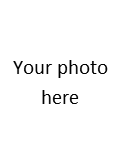
\includegraphics[width=1in,height=1.25in,clip,keepaspectratio]{a1.png}}]{First A. Author} (M'76--SM'81--F'87) and all authors may include 
biographies. Biographies are often not included in conference-related
papers. This author became a Member (M) of IEEE in 1976, a Senior
Member (SM) in 1981, and a Fellow (F) in 1987. The first paragraph may
contain a place and/or date of birth (list place, then date). Next,
the author's educational background is listed. The degrees should be
listed with type of degree in what field, which institution, city,
state, and country, and year the degree was earned. The author's major
field of study should be lower-cased. 

The second paragraph uses the pronoun of the person (he or she) and not the 
author's last name. It lists military and work experience, including summer 
and fellowship jobs. Job titles are capitalized. The current job must have a 
location; previous positions may be listed 
without one. Information concerning previous publications may be included. 
Try not to list more than three books or published articles. The format for 
listing publishers of a book within the biography is: title of book 
(publisher name, year) similar to a reference. Current and previous research 
interests end the paragraph. The third paragraph begins with the author's 
title and last name (e.g., Dr.\ Smith, Prof.\ Jones, Mr.\ Kajor, Ms.\ Hunter). 
List any memberships in professional societies other than the IEEE. Finally, 
list any awards and work for IEEE committees and publications. If a 
photograph is provided, it should be of good quality, and 
professional-looking. Following are two examples of an author's biography.
\end{IEEEbiography}

\begin{IEEEbiography}[{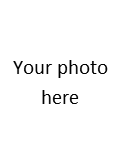
\includegraphics[width=1in,height=1.25in,clip,keepaspectratio]{a2.png}}]{Second B. Author} was born in Greenwich Village, New York, NY, USA in 
1977. He received the B.S. and M.S. degrees in aerospace engineering from 
the University of Virginia, Charlottesville, in 2001 and the Ph.D. degree in 
mechanical engineering from Drexel University, Philadelphia, PA, in 2008.

From 2001 to 2004, he was a Research Assistant with the Princeton Plasma 
Physics Laboratory. Since 2009, he has been an Assistant Professor with the 
Mechanical Engineering Department, Texas A{\&}M University, College Station. 
He is the author of three books, more than 150 articles, and more than 70 
inventions. His research interests include high-pressure and high-density 
nonthermal plasma discharge processes and applications, microscale plasma 
discharges, discharges in liquids, spectroscopic diagnostics, plasma 
propulsion, and innovation plasma applications. He is an Associate Editor of 
the journal \emph{Earth, Moon, Planets}, and holds two patents. 

Dr. Author was a recipient of the International Association of Geomagnetism 
and Aeronomy Young Scientist Award for Excellence in 2008, and the IEEE 
Electromagnetic Compatibility Society Best Symposium Paper Award in 2011. 
\end{IEEEbiography}

\begin{IEEEbiography}[{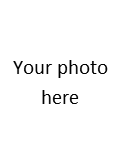
\includegraphics[width=1in,height=1.25in,clip,keepaspectratio]{a3.png}}]{Third C. Author, Jr.} (M'87) received the B.S. degree in mechanical 
engineering from National Chung Cheng University, Chiayi, Taiwan, in 2004 
and the M.S. degree in mechanical engineering from National Tsing Hua 
University, Hsinchu, Taiwan, in 2006. He is currently pursuing the Ph.D. 
degree in mechanical engineering at Texas A{\&}M University, College 
Station, TX, USA.

From 2008 to 2009, he was a Research Assistant with the Institute of 
Physics, Academia Sinica, Tapei, Taiwan. His research interest includes the 
development of surface processing and biological/medical treatment 
techniques using nonthermal atmospheric pressure plasmas, fundamental study 
of plasma sources, and fabrication of micro- or nanostructured surfaces. 

Mr. Author's awards and honors include the Frew Fellowship (Australian 
Academy of Science), the I. I. Rabi Prize (APS), the European Frequency and 
Time Forum Award, the Carl Zeiss Research Award, the William F. Meggers 
Award and the Adolph Lomb Medal (OSA).
\end{IEEEbiography}

\EOD

\end{document}
